\documentclass[11pt,oneside,openany]{book}

\usepackage[letterpaper,margin=2.25cm,headheight=15pt]{geometry}
\usepackage[T1]{fontenc}
\usepackage[utf8]{inputenc}
\usepackage{newtxtext,newtxmath}
\usepackage[scaled=0.92]{helvet}
\usepackage[scaled=0.84]{beramono}
\usepackage[spanish,es-nodecimaldot]{babel}
\usepackage{microtype}
\usepackage{amsmath}
\usepackage{booktabs,tabularx,array}
\usepackage{graphicx}
\usepackage{pdflscape}
\usepackage{xcolor}
\usepackage{enumitem}
\usepackage{listings}
\usepackage[most]{tcolorbox}
\usepackage{fancyhdr}
\usepackage{hyperref}

\definecolor{Petroleo}{HTML}{246A73}
\definecolor{Coral}{HTML}{F08A5D}
\definecolor{Tinta}{HTML}{243238}
\definecolor{Nube}{HTML}{F3F6F5}
\definecolor{Gris}{HTML}{657176}

\hypersetup{
  colorlinks=true,
  linkcolor=Petroleo,
  urlcolor=Petroleo,
  citecolor=Petroleo,
  pdftitle={Arboles de decision: guia introductoria reproducible},
  pdfauthor={Proyecto docente reproducible}
}

\pagestyle{fancy}
\fancyhf{}
\fancyhead[L]{\sffamily\small Árboles de decisión}
\fancyhead[R]{\sffamily\small Guía introductoria reproducible}
\fancyfoot[C]{\sffamily\small\thepage}
\renewcommand{\headrulewidth}{0.3pt}

\setlist{nosep,leftmargin=*}
\setlength{\parindent}{0pt}
\setlength{\parskip}{0.55em}
\renewcommand{\arraystretch}{1.18}

\lstdefinestyle{pythonstyle}{
  language=Python,
  basicstyle=\ttfamily\small,
  keywordstyle=\color{Petroleo}\bfseries,
  stringstyle=\color{Coral!80!black},
  commentstyle=\color{Gris}\itshape,
  backgroundcolor=\color{Nube},
  frame=single,
  rulecolor=\color{Petroleo!25},
  breaklines=true,
  showstringspaces=false,
  columns=fullflexible,
  keepspaces=true,
  tabsize=4,
  xleftmargin=0.4em,
  xrightmargin=0.4em
}
\lstset{style=pythonstyle}

\newtcolorbox{idea}[1][]{
  colback=Petroleo!5,
  colframe=Petroleo,
  title={#1},
  fonttitle=\sffamily\bfseries,
  boxrule=0.8pt,
  arc=2mm
}
\newtcolorbox{alerta}[1][]{
  colback=Coral!7,
  colframe=Coral!85!black,
  title={#1},
  fonttitle=\sffamily\bfseries,
  boxrule=0.8pt,
  arc=2mm
}

% Archivo generado automaticamente por scripts/run_analysis.py
\newcommand{\NTotal}{480}
\newcommand{\NTrain}{360}
\newcommand{\NTest}{120}
\newcommand{\ModelAccuracy}{0.733}
\newcommand{\ModelPrecision}{0.794}
\newcommand{\ModelRecall}{0.519}
\newcommand{\ModelFOne}{0.628}
\newcommand{\ModelAUC}{0.724}
\newcommand{\BaselineAccuracy}{0.567}
\newcommand{\TreeDepth}{3}
\newcommand{\TreeLeaves}{8}
\newcommand{\TrueNegative}{61}
\newcommand{\FalsePositive}{7}
\newcommand{\FalseNegative}{25}
\newcommand{\TruePositive}{27}


\begin{document}

\begin{titlepage}
  \pagecolor{Petroleo}
  \color{white}
  \vspace*{2.0cm}
  {\sffamily\bfseries\fontsize{34}{39}\selectfont
    Árboles de decisión\par}
  \vspace{0.5cm}
  {\sffamily\fontsize{20}{25}\selectfont
    Guía introductoria reproducible\par}
  \vspace{1.1cm}
  {\large Conceptos, código, entradas, salidas e interpretación\par}
  \vfill
  \begin{tcolorbox}[colback=white,colframe=white,arc=2mm]
    \color{Tinta}
    \textbf{Caso conductor:} clasificación de riesgo con \NTotal{} casos
    completamente simulados. Incluye un notebook ejecutable y un flujo que
    regenera todas las figuras y métricas.
  \end{tcolorbox}
  \vspace{0.8cm}
  {\sffamily\small Versión reproducible \textbullet{} septiembre de 2026}
\end{titlepage}
\nopagecolor
\color{Tinta}

\frontmatter
\chapter*{Cómo usar esta guía}
\addcontentsline{toc}{chapter}{Cómo usar esta guía}

Este texto está diseñado para una exposición introductoria de 12 a 15 minutos
y para una práctica posterior. La lectura principal explica el razonamiento; el
notebook \texttt{notebooks/01\_arboles\_decision.ipynb} permite ejecutar cada
paso y observar sus salidas.

\begin{idea}[Ruta de aprendizaje]
\textbf{Pregunta} $\rightarrow$ \textbf{división} $\rightarrow$
\textbf{árbol} $\rightarrow$ \textbf{predicción} $\rightarrow$
\textbf{evaluación} $\rightarrow$ \textbf{uso responsable}.
\end{idea}

\begin{alerta}[Alcance]
Los datos son sintéticos y no representan pacientes reales. El ejemplo enseña
un flujo de ciencia de datos; no valida una regla clínica ni autoriza decisiones
sobre personas.
\end{alerta}

\tableofcontents

\mainmatter
\chapter{Una idea sencilla: aprender preguntas}

Un árbol de decisión representa una predicción como una secuencia de preguntas.
Cada pregunta divide los datos en grupos cada vez más homogéneos. Al final de
una ruta aparece una \textbf{hoja}, que contiene la predicción.

\begin{center}
\begin{tcolorbox}[width=0.88\textwidth,colback=Nube,colframe=Petroleo!45]
\centering\sffamily
¿La edad supera un umbral?\\[0.3em]
$\swarrow$ \hspace{5cm} $\searrow$\\[-0.2em]
No: nueva pregunta \hspace{2.5cm} Sí: nueva pregunta\\[0.3em]
$\downarrow$ \hspace{5.6cm} $\downarrow$\\[-0.2em]
Hoja: clase 0 \hspace{3.4cm} Hoja: clase 1
\end{tcolorbox}
\end{center}

\section{Clasificación y regresión}

La estructura es la misma, pero cambia el tipo de respuesta:

\begin{tabularx}{\textwidth}{>{\bfseries}lXX}
\toprule
 & Clasificación & Regresión \\
\midrule
Respuesta & Categoría, por ejemplo riesgo alto/bajo & Cantidad continua, por ejemplo costo o concentración \\
Criterio típico & Gini o entropía & Error cuadrático \\
Salida de una hoja & Clase y proporción estimada & Promedio de los casos de la hoja \\
\bottomrule
\end{tabularx}

Nuestro caso es de clasificación binaria: \texttt{riesgo\_alto} vale 0 o 1.

\section{Anatomía mínima}

\begin{description}[style=nextline]
  \item[Nodo raíz] contiene todos los casos de entrenamiento y realiza la primera pregunta.
  \item[Nodo interno] realiza otra pregunta después de una división previa.
  \item[Rama] representa la respuesta verdadera o falsa a una pregunta.
  \item[Hoja] termina la ruta y entrega una predicción.
  \item[Profundidad] cuenta cuántas preguntas separan la raíz de una hoja.
\end{description}

\chapter{Cómo elige el árbol una división}

Para cada variable y varios umbrales candidatos, el algoritmo mide qué tan bien
separaría las clases. En este proyecto usamos la impureza de Gini:

\begin{equation}
G(t) = 1 - \sum_{k=1}^{K} p_{k,t}^{2},
\end{equation}

donde $p_{k,t}$ es la proporción de la clase $k$ dentro del nodo $t$. Un nodo
puro tiene $G=0$. En un problema binario, una mezcla 50/50 tiene $G=0.5$.

Para comparar una división se ponderan sus dos hijos:

\begin{equation}
G_{\mathrm{div}} = \frac{n_L}{n}G(L) + \frac{n_R}{n}G(R).
\end{equation}

El árbol selecciona la pregunta que más reduce la impureza respecto al nodo
original. Después repite el proceso dentro de cada hijo.

\begin{lstlisting}
def gini_impurity(labels):
    values, counts = np.unique(labels, return_counts=True)
    probabilities = counts / counts.sum()
    return 1.0 - np.square(probabilities).sum()
\end{lstlisting}

\begin{idea}[Ejemplo mental]
Un nodo con clases \texttt{[0, 0, 1, 1]} tiene Gini 0.5. Si una pregunta crea
dos hijos \texttt{[0, 0]} y \texttt{[1, 1]}, ambos son puros y el Gini ponderado
es 0. Esa pregunta separa perfectamente esos ocho elementos conceptuales.
\end{idea}

\section{Entropía}

Otra medida habitual es

\begin{equation}
H(t) = -\sum_{k=1}^{K} p_{k,t}\log_2 p_{k,t}.
\end{equation}

Gini y entropía suelen producir árboles parecidos. Para una introducción es más
importante comprender que ambas premian hijos homogéneos que memorizar cuál usar.

\chapter{Diseño reproducible del ejemplo}

\section{Datos de entrada}

El script \texttt{scripts/generate\_data.py} crea \NTotal{} casos con una semilla
fija. Contiene seis predictores:

\begin{tabularx}{\textwidth}{>{\ttfamily}lX}
\toprule
Variable & Interpretación pedagógica \\
\midrule
edad & años simulados \\
presion\_sistolica & medida simulada en mmHg \\
colesterol & medida simulada en mg/dL \\
fumador & indicador binario simulado \\
actividad\_horas\_semana & actividad semanal simulada \\
antecedente\_familiar & indicador binario simulado \\
\bottomrule
\end{tabularx}

\begin{figure}[htbp]
\centering
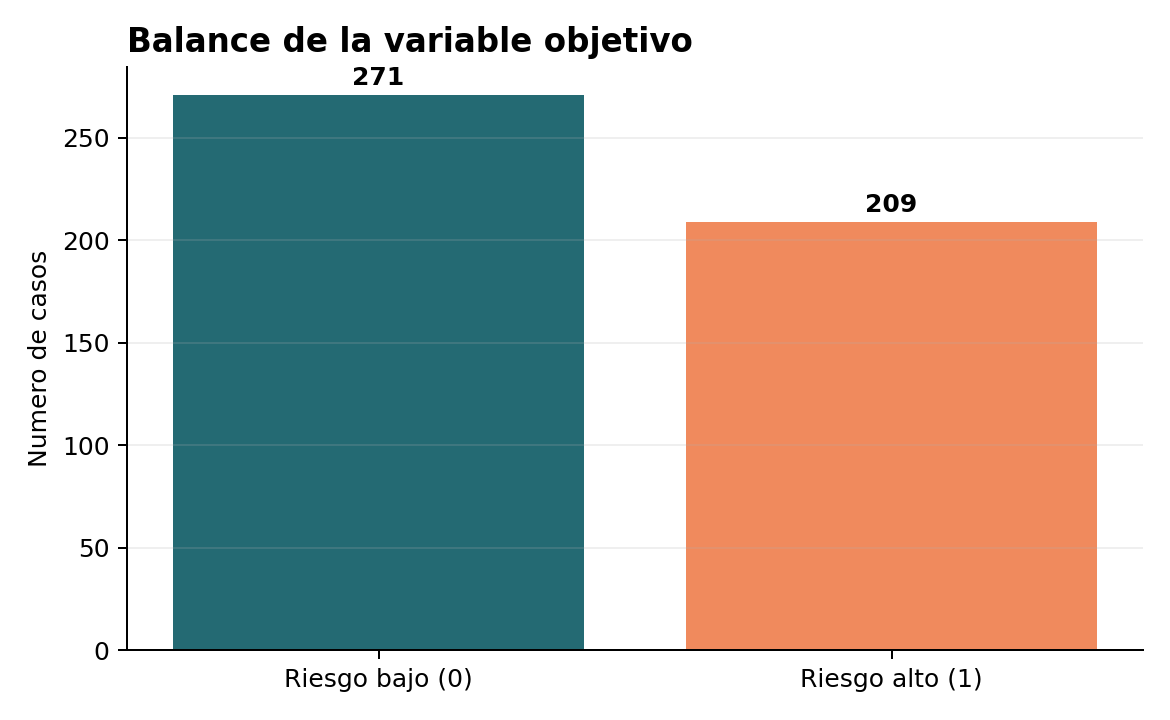
\includegraphics[width=0.72\textwidth]{../figures/class_balance.png}
\caption{Distribución de la respuesta en los datos simulados.}
\end{figure}

\section{Separación entrenamiento/prueba}

Antes de ajustar el árbol reservamos \NTest{} observaciones (25\%) para prueba y
usamos \NTrain{} para entrenamiento. La separación es estratificada, por lo que
conserva aproximadamente la proporción de clases.

\begin{lstlisting}
X_train, X_test, y_train, y_test = train_test_split(
    X, y,
    test_size=0.25,
    random_state=42,
    stratify=y,
)
\end{lstlisting}

\begin{alerta}[Fuga de información]
El conjunto de prueba simula datos nuevos. No debe utilizarse para escoger
variables, crear la respuesta, ajustar parámetros ni decidir cuándo detener el
entrenamiento. Si se usa repetidamente para tomar decisiones, deja de ser una
evaluación final independiente.
\end{alerta}

\section{Modelo deliberadamente pequeño}

\begin{lstlisting}
model = DecisionTreeClassifier(
    criterion="gini",
    max_depth=3,
    min_samples_leaf=20,
    random_state=42,
)
model.fit(X_train, y_train)
\end{lstlisting}

El árbol resultante tiene profundidad \TreeDepth{} y \TreeLeaves{} hojas. La
restricción favorece una explicación clara, pero en una aplicación real estos
valores deben justificarse mediante validación y conocimiento del problema.

\chapter{El árbol y sus reglas}

Para leer un nodo:

\begin{enumerate}
  \item comprobar la pregunta de la primera línea;
  \item ir a la izquierda si es verdadera y a la derecha si es falsa;
  \item observar \texttt{samples} y \texttt{value} para saber cuántos casos llegaron;
  \item continuar hasta una hoja y leer la clase mayoritaria.
\end{enumerate}

\begin{idea}[Regla, no explicación causal]
Una ruta describe cómo este modelo asigna una predicción. No prueba que cambiar
una variable cause un cambio en el desenlace. Asociación predictiva y causalidad
son preguntas diferentes.
\end{idea}

\begin{landscape}
\begin{figure}[p]
\centering
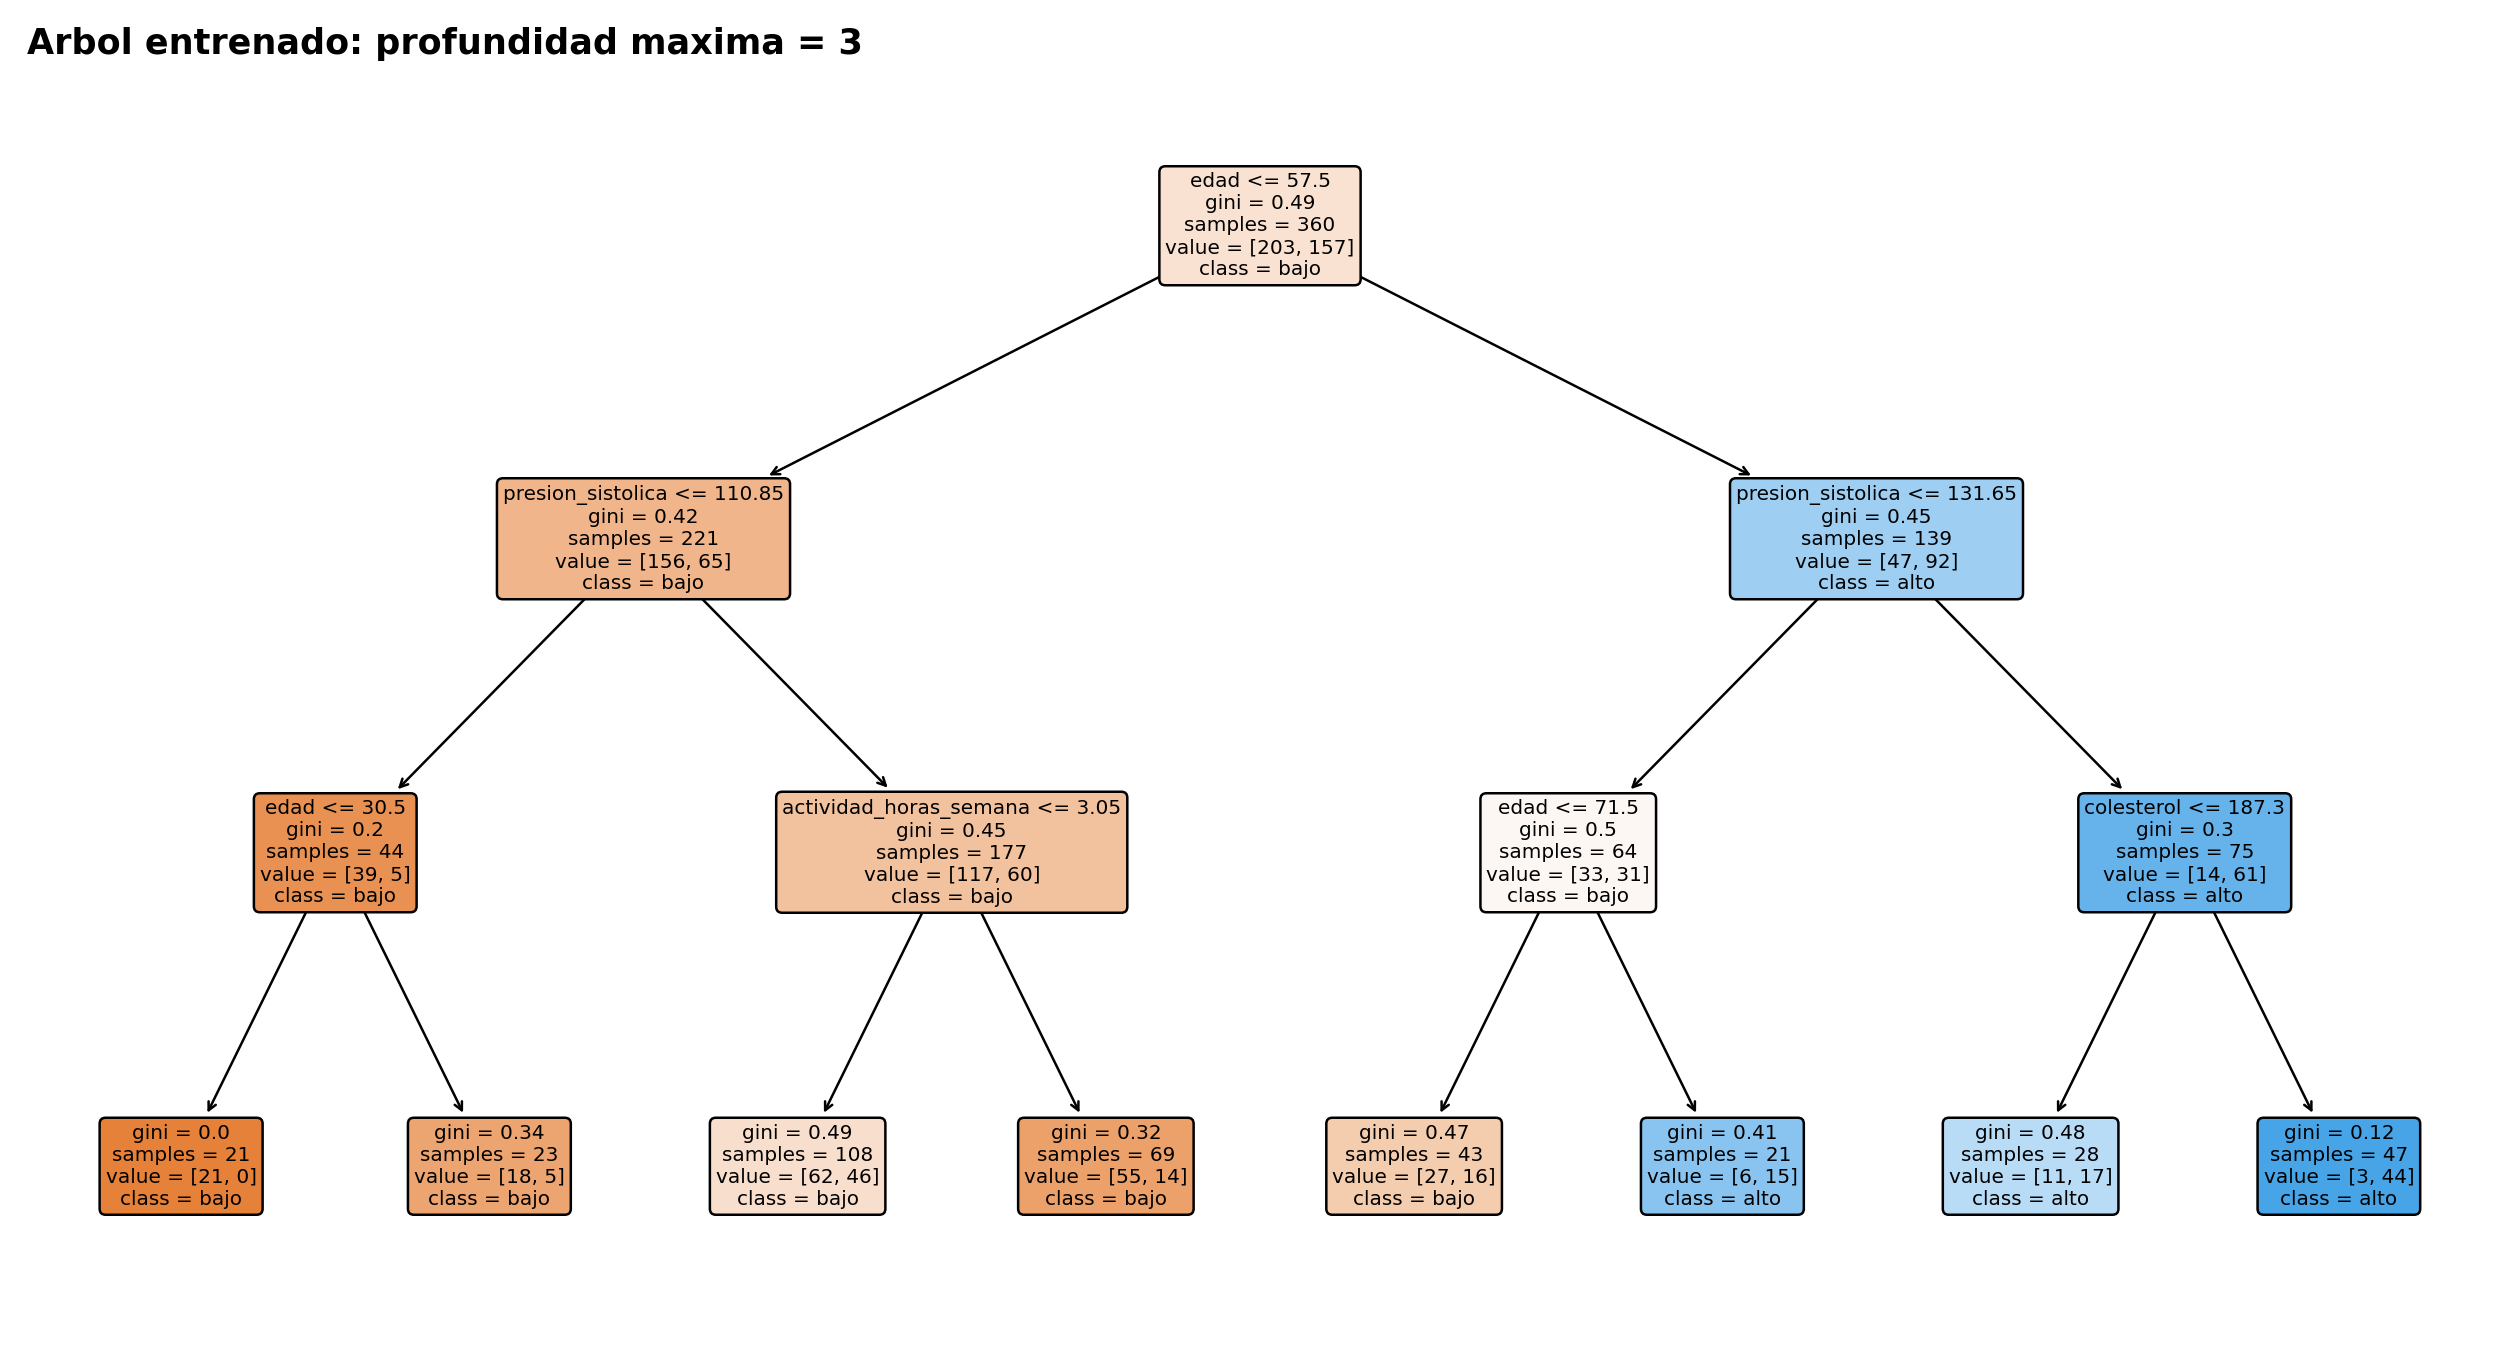
\includegraphics[width=0.96\linewidth]{../figures/decision_tree.png}
\caption{Árbol aprendido únicamente con el conjunto de entrenamiento. Los
colores indican la clase dominante, no certeza causal.}
\end{figure}
\end{landscape}

\chapter{Entradas, salidas y evaluación}

El siguiente fragmento produce probabilidades, clases y métricas sobre el
conjunto que el árbol no vio durante el ajuste:

\begin{lstlisting}
prediction = model.predict(X_test)
probability = model.predict_proba(X_test)[:, 1]

accuracy = accuracy_score(y_test, prediction)
precision = precision_score(y_test, prediction)
recall = recall_score(y_test, prediction)
roc_auc = roc_auc_score(y_test, probability)
\end{lstlisting}

\section{Resultados reproducidos}

\begin{tabular}{lr}
\toprule
Métrica & Valor en prueba \\
\midrule
Exactitud & \ModelAccuracy \\
Precisión & \ModelPrecision \\
Sensibilidad (recall) & \ModelRecall \\
F1 & \ModelFOne \\
ROC AUC & \ModelAUC \\
Referencia: clase mayoritaria & \BaselineAccuracy \\
\bottomrule
\end{tabular}

La exactitud supera la referencia ingenua que siempre predeciría la clase más
frecuente. Aun así, la sensibilidad muestra que algunos casos positivos no son
detectados. El modelo es útil para enseñar la evaluación precisamente porque no
es perfecto.

\section{Matriz de confusión}

\begin{center}
\begin{tabular}{lcc}
\toprule
 & Predicho 0 & Predicho 1 \\
\midrule
Observado 0 & \TrueNegative & \FalsePositive \\
Observado 1 & \FalseNegative & \TruePositive \\
\bottomrule
\end{tabular}
\end{center}

\begin{figure}[htbp]
\centering
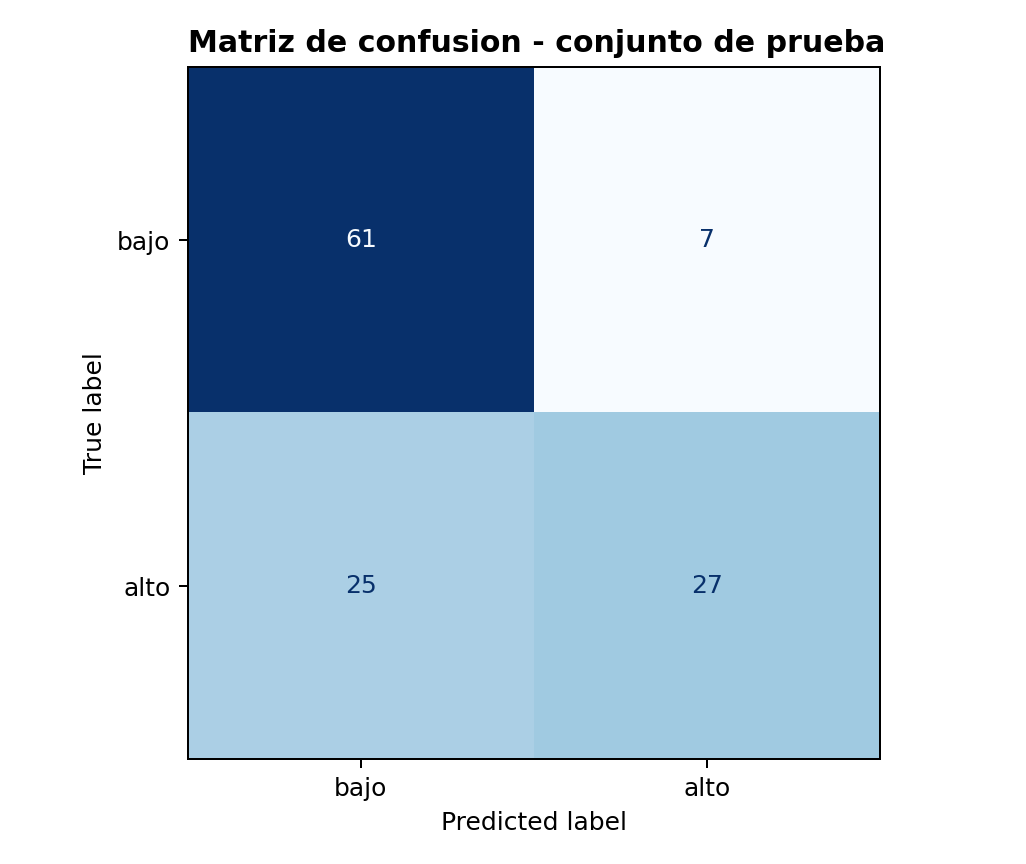
\includegraphics[width=0.62\textwidth]{../figures/confusion_matrix.png}
\caption{Cada celda corresponde a un tipo de acierto o error.}
\end{figure}

\section{Ejemplos de entrada y salida}

Estas filas proceden del CSV de predicciones generado por el pipeline:

\begin{center}
\small
\begin{tabular}{rrrrrrr}
\toprule
ID & Edad & PAS & Fuma & Obs. & Pred. & $P(y=1)$ \\
\midrule
% Archivo generado automaticamente
10 & 69 & 129.9 & 0 & 0 & 0 & 0.372 \\
11 & 50 & 134.9 & 1 & 0 & 0 & 0.426 \\
19 & 41 & 125.6 & 0 & 0 & 0 & 0.426 \\
21 & 51 & 152.2 & 0 & 0 & 0 & 0.426 \\
24 & 32 & 148.5 & 0 & 0 & 0 & 0.426 \\
28 & 23 & 113.7 & 0 & 0 & 0 & 0.426 \\
\bottomrule

\end{tabular}
\end{center}

La probabilidad es la proporción de clase 1 observada en la hoja correspondiente.
En árboles pequeños puede repetirse para muchos casos y no debe interpretarse
automáticamente como una probabilidad clínicamente calibrada.

\begin{figure}[htbp]
\centering
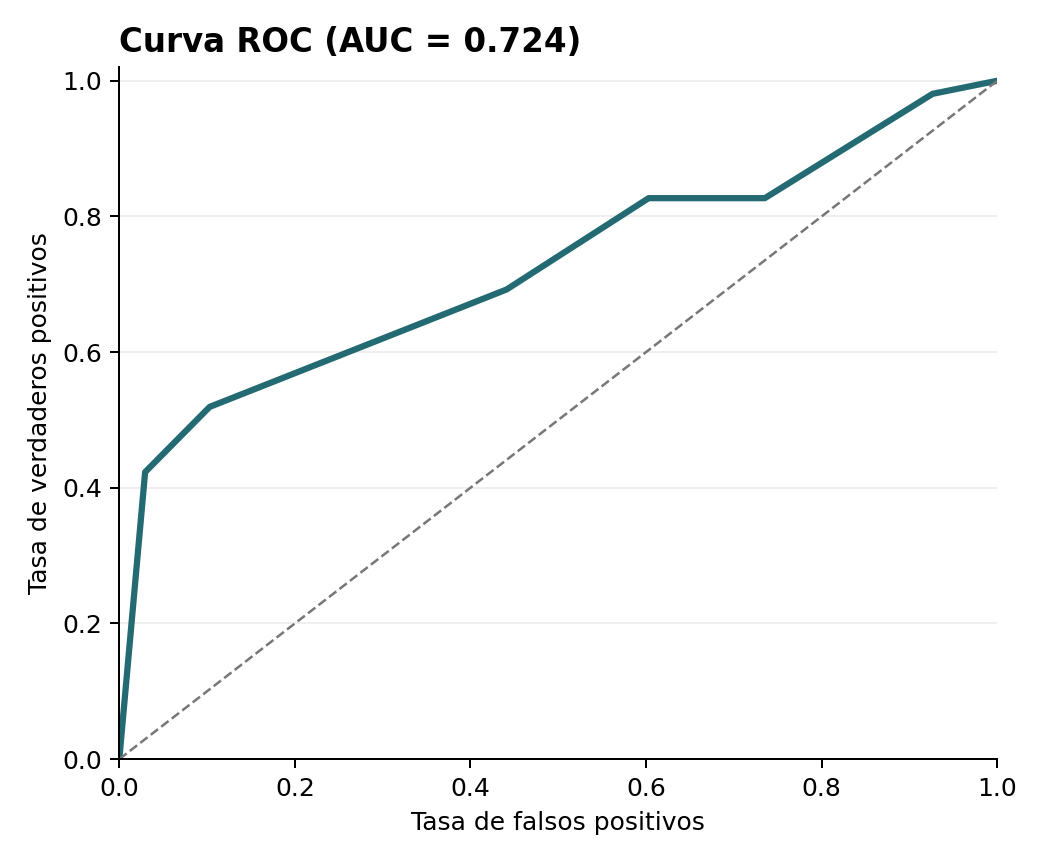
\includegraphics[width=0.64\textwidth]{../figures/roc_curve.png}
\caption{La curva ROC resume el intercambio entre sensibilidad y falsos
positivos a través de varios umbrales.}
\end{figure}

\chapter{Complejidad, poda y sobreajuste}

Un árbol sin restricciones puede continuar dividiendo hasta memorizar detalles
del entrenamiento. Esto reduce el error aparente, pero las reglas pueden ser
inestables y generalizar peor.

\begin{figure}[htbp]
\centering
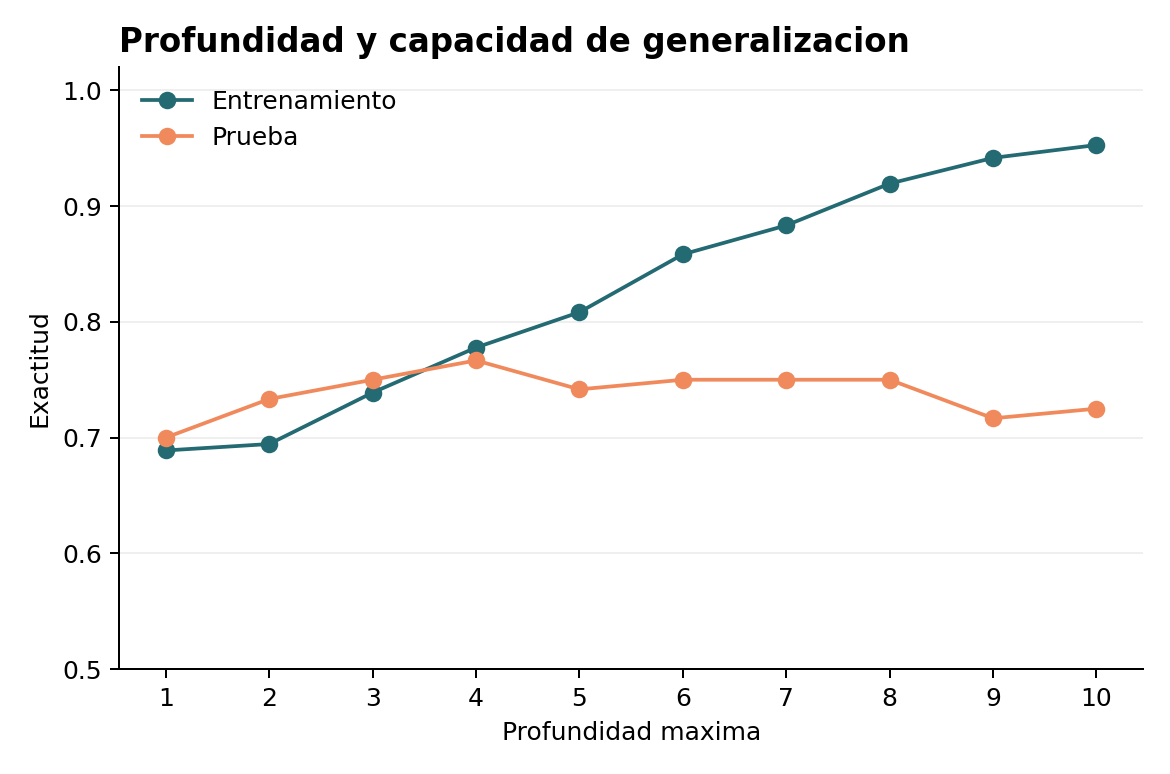
\includegraphics[width=0.64\textwidth]{../figures/depth_curve.png}
\caption{La exactitud de entrenamiento crece con la profundidad; la de prueba
no tiene por qué hacerlo. Esta comparación es ilustrativa, no sustituye la
validación cruzada.}
\end{figure}

Dos familias de control son:

\begin{description}[style=nextline]
  \item[Pre-poda] limitar profundidad, número de hojas o tamaño mínimo de hoja
  antes y durante el crecimiento.
  \item[Post-poda] crecer un árbol y retirar ramas cuyo beneficio no compensa su
  complejidad. CART formaliza esta idea mediante poda por costo-complejidad.
\end{description}

Una forma conceptual del criterio es

\begin{equation}
R_{\alpha}(T) = R(T) + \alpha |T|,
\end{equation}

donde $R(T)$ mide el error, $|T|$ la cantidad de hojas y $\alpha$ penaliza la
complejidad. Un $\alpha$ mayor favorece árboles más pequeños.

\chapter{Interpretación responsable}

\begin{figure}[htbp]
\centering
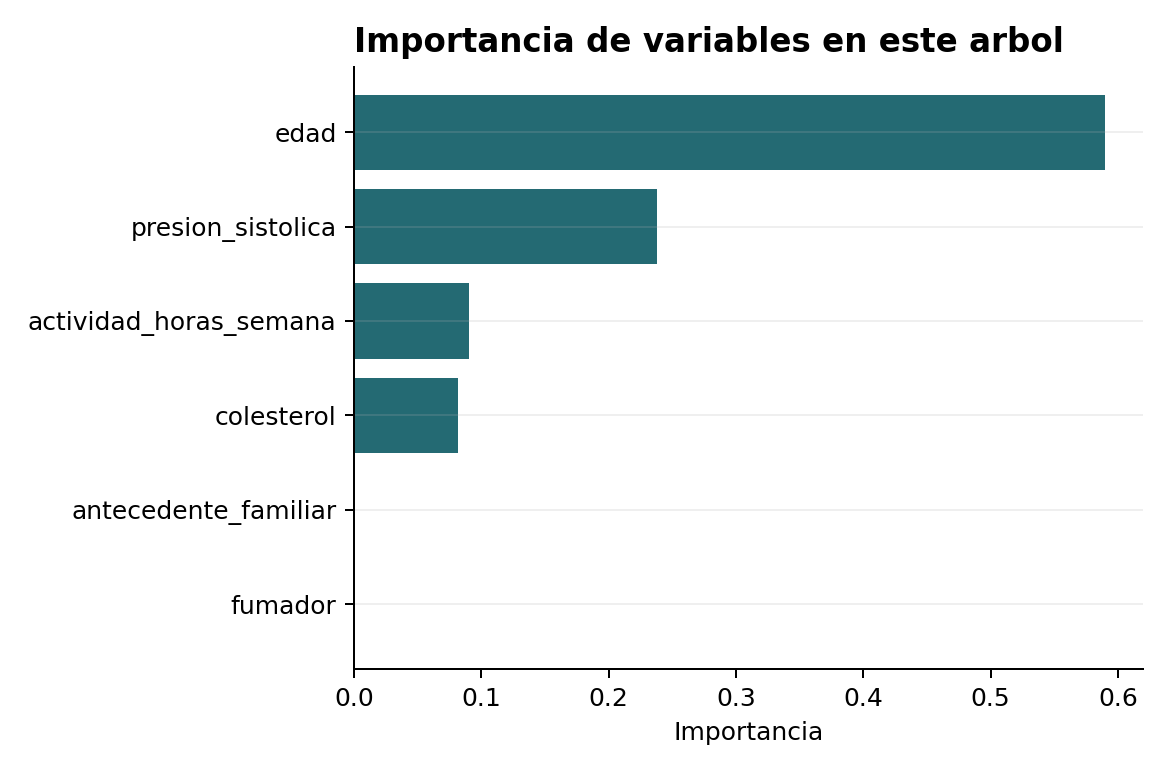
\includegraphics[width=0.76\textwidth]{../figures/feature_importance.png}
\caption{Importancia basada en reducción de impureza dentro de este modelo.}
\end{figure}

La importancia indica cuánto contribuyó una variable a reducir la impureza en
este árbol. No representa un efecto causal y puede favorecer variables con más
oportunidades de división. Las variables correlacionadas también pueden
repartirse o intercambiar importancia.

\section{Ventajas}

\begin{itemize}
  \item reglas visuales y fáciles de comunicar;
  \item relaciones no lineales e interacciones sin especificarlas a mano;
  \item poca preparación numérica para un ejemplo tabular limpio;
  \item aplicable a clasificación y regresión.
\end{itemize}

\section{Limitaciones}

\begin{itemize}
  \item alta variabilidad: cambios pequeños pueden producir otro árbol;
  \item sobreajuste si no se controla la complejidad;
  \item divisiones codiciosas que no garantizan el árbol globalmente óptimo;
  \item probabilidades por hoja potencialmente poco calibradas;
  \item sesgos de los datos se trasladan a las reglas y resultados.
\end{itemize}

\begin{alerta}[Antes de cualquier uso real]
Se requieren datos representativos, definición clínica válida del desenlace,
tratamiento documentado de faltantes, validación cruzada, evaluación externa,
análisis por subgrupos, calibración y revisión ética/profesional. Nada de eso
puede inferirse de este caso sintético.
\end{alerta}

\chapter{Guion breve para exponer}

\begin{tabularx}{\textwidth}{>{\bfseries}p{1.8cm}X}
\toprule
Tiempo & Mensaje sugerido \\
\midrule
0--2 min & Un árbol convierte una predicción en una secuencia de preguntas. Presentar raíz, ramas, nodos y hojas. \\
2--4 min & Distinguir clasificación y regresión. Explicar que nuestro desenlace es binario y simulado. \\
4--6 min & Mostrar Gini intuitivamente: una hoja pura tiene valor 0; una mezcla 50/50 es más impura. \\
6--8 min & Explicar separación entrenamiento/prueba y por qué evita evaluar con los mismos casos usados para aprender. \\
8--11 min & Recorrer una ruta del árbol y mostrar la matriz de confusión. Contrastar exactitud con sensibilidad. \\
11--13 min & Mostrar sobreajuste, profundidad y poda. \\
13--15 min & Resumir ventajas, límites y condiciones necesarias para un uso responsable. \\
\bottomrule
\end{tabularx}

\section{Preguntas frecuentes}

\textbf{¿Gini o entropía?} Ambas miden mezcla y suelen dar resultados similares.
Conviene comparar dentro de una validación, no escoger por costumbre.

\textbf{¿Por qué no usar todos los datos para entrenar?} Porque necesitamos una
estimación del comportamiento ante casos no vistos.

\textbf{¿La variable más importante es la causa principal?} No. La importancia
describe el uso predictivo dentro del árbol y los datos observados.

\textbf{¿Por qué limitar la profundidad?} Para controlar sobreajuste, estabilidad
y facilidad de interpretación.

\textbf{¿Un árbol interpretable es automáticamente confiable?} No. Las reglas
pueden ser transparentes y, al mismo tiempo, estar sesgadas o no generalizar.

\chapter{Reproducir el proyecto}

Desde la raíz del repositorio:

\begin{lstlisting}[language=bash]
conda env create -f environment.yml
conda activate arboles-decision
make all
\end{lstlisting}

El flujo sigue este orden:

\begin{enumerate}
  \item \texttt{scripts/generate\_data.py} crea el CSV de entrada;
  \item \texttt{scripts/run\_analysis.py} ajusta el árbol y genera métricas,
  predicciones, reglas, tablas y figuras;
  \item Jupyter ejecuta el notebook y guarda las salidas;
  \item Tectonic compila esta guía incorporando los resultados generados;
  \item las pruebas verifican Gini, la separación y propiedades básicas del modelo.
\end{enumerate}

\begin{idea}[Una sola fuente de verdad]
La lógica del modelo vive en \texttt{src/arboles\_decision/pipeline.py}. El
notebook, los scripts y el PDF consumen esa misma implementación. Así se reduce
el riesgo de presentar números distintos a los que produce el código.
\end{idea}

\backmatter
\chapter{Referencias y lecturas}

\begin{itemize}
  \item Breiman, L., Friedman, J. H., Olshen, R. A., y Stone, C. J. (1984).
  \emph{Classification and Regression Trees}. Wadsworth.
  \item Ma, X. (2018). \emph{Using Classification and Regression Trees: A
  Practical Primer}. Information Age Publishing. Capítulo 3, pp. 39--47.
  \item Pedregosa, F. et al. (2011). Scikit-learn: Machine Learning in Python.
  \emph{Journal of Machine Learning Research}, 12, 2825--2830.
\end{itemize}

\chapter*{Lista de comprobación final}
\addcontentsline{toc}{chapter}{Lista de comprobación final}

\begin{itemize}
  \item[$\square$] Puedo explicar una ruta desde la raíz hasta una hoja.
  \item[$\square$] Puedo calcular Gini en un ejemplo pequeño.
  \item[$\square$] Distingo entrenamiento, validación y prueba.
  \item[$\square$] Interpreto los cuatro cuadrantes de la matriz de confusión.
  \item[$\square$] Sé por qué exactitud no siempre es suficiente.
  \item[$\square$] Puedo explicar sobreajuste y dos formas de controlarlo.
  \item[$\square$] No confundo importancia predictiva con causalidad.
  \item[$\square$] Puedo declarar claramente que el caso es sintético y educativo.
\end{itemize}

\end{document}
